\chapter{Interactive obstruction-free lensing for volumetric data visualization}
\label{lensing}

Occlusion is an issue in volumetric visualization as it prevents direct visualization of the region of interest. While many techniques such as transfer functions, volume segmentation or view distortion have been developed to address this, there is still room for improvement to better support the understanding of objects' vicinity. However, most existing Focus+Context fail to solve partial occlusion in datasets where the target and the occluder are very similar density-wise. For these reasons, we investigate a new technique which maintains the general structure of the investigated volumetric dataset while addressing occlusion issues. With our technique, the user interactively defines an area of interest where an occluded region or object is partially visible. Then our lens starts pushing at its border occluding objects, thus revealing hidden volumetric data. Next, the lens is modified with an extended field of view (fish-eye deformation) to better see the vicinity of the selected region. Finally, the user can freely explore the surroundings of the area under investigation within the lens. To provide real-time exploration, we implemented our lens using a GPU accelerated ray-casting framework
to handle ray deformations, local lighting, and local viewpoint manipulation. We illustrate our technique with five application scenarios in baggage inspection, 3D fluid flow visualization, chest radiology, air traffic planning, and DTI fiber exploration.

\section{Introduction}
Direct volume rendering (DVR) is a pervasive visualization technique for displaying 3D scalar fields with applications in engineering, material sciences, and medical imaging sciences. However widely adopted, and able to handle large datasets at interactive rates, DVR inherently suffers from the problem of \emph{occlusion}: Structures of interest located deep in the volume, called next \emph{targets}, can be hard to spot and/or explore.

To aid with this, various techniques have been designed including transfer functions, segmentation, selection, and clipping. Yet, all such techniques have limitations.  \emph{Global} mechanisms, like transfer function editing, can remove both occluders and targets if these have similar densities. In certain applications, carefully designed transfer functions exist and should be used without (significant) modifications to facilitate understanding and user training\,\cite{4276082}. \emph{Local} mechanisms like segmentation, selection, or clipping are more effective in manipulating data confined to a given spatial region. Yet, many such mechanisms assume that one can easily and accurately select targets to remove them (occluders) or keep them (occluded). This is hard to do when \emph{e.g.} one does not have direct access to the targets, or when significant 3D interaction is required to select occluder(s).

A different way to handle occlusion is to use \emph{lenses}. These are flexible lightweight tools which enable local and temporary modifications of the DVR to reveal targets while keeping the global visualization context, \cite{595268,CGF:CGF12871,6327262}. However, efficiently selecting the target and  removing all in-between occluders is still challenging. More specifically, most existing occlusion management techniques do not simultaneously meet all following requirements: Rapidly create an unobstructed view of the target (R1), allow a flexible local exploration of the target zone (R2), keep the context in which the target is visually embedded (R3), and handle datasets where the target and occluders cannot 
be separated by transfer function manipulations (R4).

In this chapter, we increase the flexibility of lenses for DVR exploration to jointly cover all above requirements. We propose a focus-and-context (F+C) lens that combines a distortion technique, which pushes aside the occluding objects, with a fish-eye field of view, to provide a better perspective on targets. We specifically target the use-case of \emph{partially occluded} objects, where the user has a glimpse of an interesting structure, buried deep in the data, but only slightly visible from a given viewpoint and transfer-function setting. We allow the user to ''open up'' the volume without changing these settings, and reveal the target, by simple point, click, and scroll operations. Next, we provide several F+C modifications of the lighting parameters, transfer function, and geometry in the focus area to better understand the target. Our technique, implemented using a CUDA-based approach, can be easily incorporated in any generic DVR system.

The chapter is structured as follows. \autoref{sec:requirements} presents again the four requirements for occlusion management in DVR visualization. \autoref{sec:principle} introduces the principle of our lens. \autoref{sec:implem} introduces implementation details.\autoref{sec:scenarios} presents five application scenarios for our lens in baggage inspection, 3D fluid flow visualization, chest radiology, air traffic planning, and DTI fiber exploration. \autoref{sec:discussion} discusses our proposal. Finally, Section~\autoref{sec:conclusions} concludes the chapter.

\section{Requirements}
\label{sec:requirements}

To start with, let us recall requirements R1$,\ldots,$R4.
\begin{itemize}
\item{\textbf{R1:}} The technique should rapidly create an unobstructed view of the target, \emph{i.e.}, such a view should be created at interactive frame rates (10 fps or more) with no special pre-processing of the input volume (\emph{e.g.}, segmentation), and with minimal user input (\emph{e.g.}, using simple mouse and/or keyboard-modifier events). All above are needed to ensure that one can freely \emph{explore} the volume by activating the lens anywhere with minimal effort and seeing its effect in real-time.

\item{\textbf{R2:}} Allowing a flexible exploration of the target zone means that one can manipulate the zone in the lens in various ways to see how the target is actually embedded in its surrounding context.

\item{\textbf{R3:}} Keeping the context means that the visualization around the lens does not change significantly from what would be shown there if the lens were not activated. This is needed to maintain the user's mental map before \emph{vs} after activating the lens.

\item{\textbf{R4:}} The lens should enable the exploration of datasets where targets cannot be easily separated (isolated) from their surrounding context simply by manipulating parameters of the transfer functions (TF). One such issue is when targets and surrounding zones have similar densities; in this case, using a single global opacity TF could either render everything opaque (thus, it will be hard to visually isolate the target) or highly transparent (thus, the zone around the target will be transparent but so will be the target too).
\end{itemize}





\subsection{Detailed contributions}
%
Summarizing the above discussion on the requirements and related work on occlusion management, we propose a new technique which combines high-quality DVR with a fast, versatile, and easy to use, lens to support the interactive exploration of occluded data in volumes. In the classification of view deformations by C\cite{595268}, we use a nonlinear radial distortion through an interactive lens to remove occluding items and keep the global context while magnifying a partially occluded item. Related to volumetric lens techniques, we frame our contribution as follows: We propose an interactive deforming lens that magnifies and pushes aside occluding objects located in front of a designated focal point which meets the four requirements; the combination of flexible and real-time interactive changing of the focal point, custom bent rays used for DVR, lens deformation, and shading and transfer function in the focus area allow us to provide \emph{on the fly} a range of perspectives of the targets, without having to change the viewpoint or manipulate complex parameters in multiple linked views.


\begin{figure}
\centering

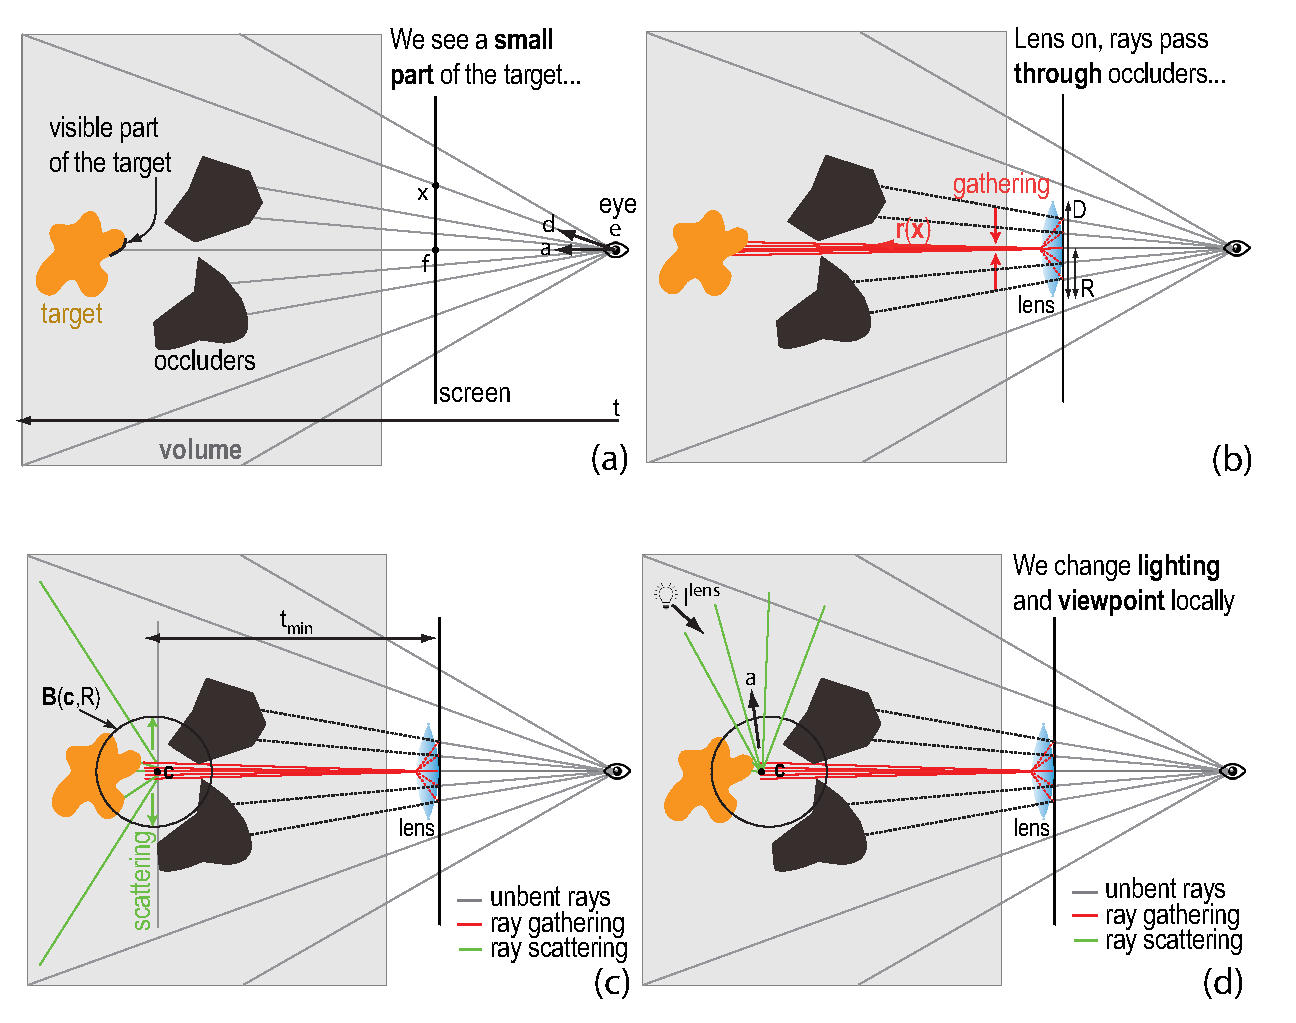
\includegraphics [width=\textwidth]{images/principle.eps}

\caption[Obstruction-free lens working.]{Obstruction-free lens working. A target is (mostly) hidden by occluders in front of it. (a) Classic DVR shows a small part of the target. (b) Our lens gathers rays to avoid occluders (\autoref{sec:gathering}). Once close to the target, rays follow again their initial paths. Yet, only a small part of the target is visible. (c) Scattering rays makes the full target visible (\autoref{sec:scattering}). Finally, we adjust the local viewing and lighting directions $\mathbf{a}$, $\mathbf{l}^{lens}$ (\autoref{sec:inter_expl}).}
\label{f:fisheye}

\end{figure}
\section{Principle}
\label{sec:principle}
%
%
Consider the typical DVR algorithm: Given a scalar volume $V \subset \mathbf{R}^3 \rightarrow \mathbf{R}$, each pixel $\mathbf{x} \in I$ in the DVR image $I \subset \mathbf{R}^2$ thereof corresponds to the compositing of sampled data along a ray that passes through $V$ and ends at $\mathbf{x}$. In classical DVR (\autoref{f:fisheye}-a), such rays are defined by the eye position $\mathbf{e}$ and a ray direction unit vector
\begin{equation}
\mathbf{d} = \frac{ (\mathbf{x} - \mathbf{e}) }{ \| \mathbf{x} - \mathbf{e} \| }
\end{equation}
. Consider now a focus point $\mathbf{f} \in I$ (the lens center) and a lens radius $R > 0$. We modify all rays passing through the lens (focus/0 area $D = \{\mathbf{x} \in I | \| \mathbf{x} - \mathbf{f} \| \leq R\}$ in order to de-occlude, magnify, and emphasize a target object. Our ray behavior is divided into three steps: (1) Provide a clear view of the target by moving closer to it and by pushing occluders aside. (2) Set a wide field-of-view (fisheye) to better see the target. (3) Modify the parameters of the lens, lighting, and opacity TF in real time to better explore the target. These steps are detailed next.

\subsection{Creating an unobstructed view}
\label{sec:gathering}
%
The scenario we address is as follows: Given a volume $V$, users produce a DVR thereof, using whatever suitable TFs and other parameters are applicable. When examining $V$ from various viewpoints, (at least) one viewpoint $(\mathbf{e},\mathbf{d})$ is found from which some intriguing structure is \emph{partially} visible in $I$. We call this structure the \emph{target}. Users next want to quickly and easily unravel the target. For this, we proceed as follows: We first \emph{gather} all rays passing through the lens pixels (focus area $D$) to follow the lens' axis vector

\begin{equation}
 \mathbf{a} = \frac{ (\mathbf{f} - \mathbf{e}) } { \| \mathbf{f} - \mathbf{e} \| }
 \end{equation}
 . As explained above, at the location $\mathbf{f}$ of the lens center, we do see an interesting partially occluded target. Hence, by definition, the gathered rays pass \emph{through} occluders to hit this target, otherwise we would not see it. We control gathering by setting the ray direction passing through $\mathbf{x} \in D$ to
%
\begin{equation}
\mathbf{r}(\mathbf{x}) = (1-\alpha) \mathbf{a} + \alpha \mathbf{d},
\label{eqn:gathering}
\end{equation}
%
with $\alpha \in [0,1]$. When $\alpha=0$ (default), all rays follow the lens axis $\mathbf{a}$, thus, can best pass through obstacles. When $\alpha=1$, rays follow a straight path. Changing $\alpha$ with the mouse wheel smoothly navigates between the lens effect, \emph{i.e.} opening up a 'hole' in the volume to see the target, and classical DVR.
%
\subsection{Setting a wide field of view}
\label{sec:scattering}
%
Once the rays pass obstacles (\autoref{sec:gathering}), we want to \emph{scatter} them so as to best sample the target. Consider that this target is at some depth $t_{target}>0$ within $V$. After the rays pass the occluders, but before they hit the target, \emph{i.e.}, travel past a distance $t_{min} < t_{target}$ through $V$, we deflect (scatter) them so as to best sample the target. For this, we set the parametric position of a ray point to
%
\begin{equation}
\mathbf{p}(\mathbf{x}, t) = \mathbf{r}(\mathbf{x})t + \beta (\mathbf{x}-\mathbf{f})(t-t_{min})
\label{eqn:scattering}
\end{equation}
%
for any pixel $\mathbf{x} \in D$ and any $t \geq t_{min}$. Here, $\beta \geq 0$, adjusted via the mouse scroll wheel while pressing the Shift key (\autoref{f:fisheye}-c), controls the ray scattering: Small values magnify a small volume area close to the ray $\mathbf{r}(\mathbf{x})$; larger values sample more of the volume behind the lens. Intuitively, this is as if we moved a magnifying lens to a depth $t_{min}$ inside $V$. Summarizing, after the user finds an interesting but partially occluded target using \emph{standard} DVR, our lens squeezes rays to pass between occluders and next fans them out to explore the target.
%
%


\subsection{Interactive exploration of the target}
\label{sec:inter_expl}
%
To achieve a more effective exploration, we can interactively modify several parameters of the DVR and the lens, as follows.
%
\begin{figure}
\centering

\includegraphics [width=\textwidth]{images/params.eps}

\caption[Changing lighting parameters in the lens.]{Changing lighting parameters in the lens. (a) Constant global specular coefficient. (b) Specular coefficient high in the lens and low outside. (c-f) Changing the in-lens light vector yields the effect of a flashlight rotating around the target. The ball icons illustrate the local light vector direction.}
\label{f:params}

\end{figure}
%



\par \textbf{Lens radius:} The radius $R$, telling how big is the 'hole' to open up in the volume to see the target, is set via the mouse wheel. The parameters $\alpha$ and $\beta$ (affecting the gathering and scattering of rays respectively) are set by the mouse wheel and modifier keys. The value $t_{min}$ (depth from which scattering starts) is set using the arrow keys.

\par  \textbf{Lens axis:} Users can rotate the lens axis $\mathbf{a}$ using a virtual trackball activated by the right mouse button. Changing $\mathbf{a}$ effectively samples the target from many viewpoints, allowing the user to look 'around' it to see parts which are not visible from the current viewpoint, but \emph{without} actually changing the viewpoint. This is of high added value, since changing the viewpoint can bring us to a view where the target is fully invisible, so we do not know where precisely to activate the lens anymore. \autoref{f:rotation} shows three such local rotations for the baggage dataset introduced in  \autoref{f:baggage_lens}. From these, we see that the star-shaped target is relatively thick.


\par  \textbf{Lighting:} We modify the volumetric Phong lighting parameters to better explore the target, as follows. Let
\begin{equation}
\mathbf{c} = \mathbf{e} + t_{min}\mathbf{a}
\end{equation} 
 be a point at depth $t_{min}$ along the lens axis, and let $B(\mathbf{c},R)$ be a sphere of radius $R$ around this point (\autoref{f:fisheye}b). We call voxels in this sphere 'in focus', and all other voxels in $V$ 'out of focus'. Let $\phi$ be the specular term coefficient, set to a high value (default: one).
First, for all voxels $\mathbf{x} \in B(\mathbf{c},R)$, we use a specular coefficient 
\begin{equation}
\phi(\mathbf{x}) = \phi (1-d)
\end{equation}
, where 
\begin{equation}
 d= \frac{\|\mathbf{x}-\mathbf{c}\|}{R}
\end{equation}. 
For all voxels outside $B(\mathbf{c},R)$, we use $\phi(\mathbf{x}) = 0$. Hence, voxels close to the focus point $\mathbf{c}$ appear highly specular; further away from $\mathbf{c}$, voxels get less specular, and voxels out of focus are purely diffuse. Secondly, we allow the user to locally rotate the light vector using the same trackball mechanism as for the lens axis rotation. Let $\mathbf{l}^{lens}$ be this vector, and let $\mathbf{l}^{global}$ be the global light vector used by standard DVR. For all voxels in focus, we use a light vector
\begin{equation}
\mathbf{l}(\mathbf{x}) = (1 - d)\mathbf{l}^{lens} + d\mathbf{l}^{global}
\end{equation}.
 
  As the user rotates $\mathbf{l}^{lens}$, the light direction will visibly change in the middle of the lens, stay constant outside it, and smoothly change in between.


\par  The above two mechanisms combined yield the effect of a moving flashlight turning around a shiny target embedded in a constantly-lit diffuse scene. \autoref{f:params} shows these mechanisms for a chest CT dataset containing a deeply buried tumor (the dataset and use-case are described in detail in \autoref{sec:chest}). We see how turning the light highlights small-scale details on the target surface (tumor) without changing the viewpoint or lens location. Moreover, the high specularity in the lens attracts the user's attention to this area; the diffuse lighting outside the lens put less emphasis on the context area. 


\par  \textbf{Opacity:} We modify the opacity transfer function along a similar idea as for lighting ( \autoref{fig:tf}). Let $TF_{o}^{global} : \mathbf{R} \rightarrow [0,1]$ be the user-chosen opacity function used globally for the volume. Let $\Gamma$ be a Gaussian pulse of unit height centered at the average density value $\bar{\rho}$ in $B(\mathbf{c},R)$ and with standard deviation $\sigma$. We estimate $\bar{\rho}$ and $\sigma$ by considering the density $\rho$ at 150 points randomly sampled inside $B(\mathbf{c},R)$. Higher values for the sample count yield visually very similar results for our tested volumes of up to $500^3$ voxels, while requiring (slightly) more computation costs. Then, for voxels in $B(\mathbf{c},R)$, we use an effective opacity transfer function   
\begin{equation}
TF_o = TF_{o}^{global} + (1-d) \Gamma
\end{equation}.
 For voxels outside $B$, we use $TF_{o}^{global}$ (standard DVR).
This is useful when the user sets $TF_{o}^{global}$ to make most out-of-lens voxels relatively transparent. In that case, $TF_o$ will still make voxels in $B$ opaque, thus allowing to see the in-focus structures better. \autoref{f:params} has been generated this way.


%ALEX: This phrase was indeed confusing, I don't know what we wanted to say with it: 
%We see here how the tumor in the lens has the same opacity as the muscle tissue outside the lens, even though the two have nearly identical densities.

\begin{figure}
\centering
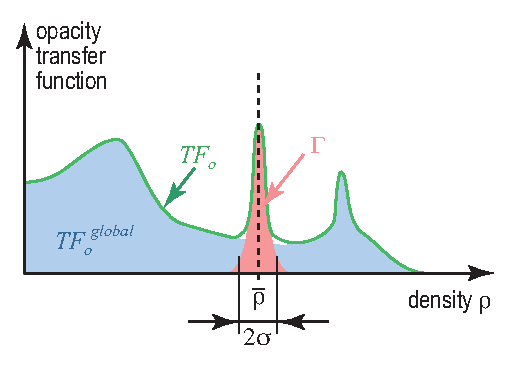
\includegraphics[width=0.95\textwidth]{images/tf.eps}

\caption{Construction of local transfer function $TF_{o}$. See \autoref{sec:inter_expl}.}

\label{fig:tf}
\end{figure}


\subsection{Smooth transitions}
\label{continuity} 
%
If we bend rays passing through the lens pixels $D$ (\autoref{eqn:gathering} and \autoref{eqn:scattering}) and trace rays starting at pixels in $I \setminus D$ as straight lines, discontinuities appear at the lens borders. We solve this as follows. Let $\mathbf{p}(\mathbf{x},t)$ be the voxels along a lens ray starting at screen pixel $\mathbf{x}$, as computed by  \autoref{eqn:scattering}. Let $\mathbf{p}^{line}(\mathbf{x},t)$ be the voxels along a straight-line ray starting at $\mathbf{x}$, \emph{i.e.}, computed using $\alpha=1$ and $\beta=0$ in  \autoref{eqn:gathering} and \autoref{eqn:scattering} respectively. For every value $t$ along every such ray, we compute the interpolated ray
\begin{equation}
\bar{\mathbf{p}}(\mathbf{x},t) = (1-f(d))\mathbf{p}(\mathbf{x},t) + f(d)\mathbf{p}^{line}(\mathbf{x},t)
\end{equation},
 where $d$ is the distance of $\mathbf{x}$ to the lens axis (normalized to unit by dividing it by $R$) and $f : [0,1] \rightarrow [0,1]$ is an interpolation function. Next, we use the rays $\bar{\mathbf{p}}(\mathbf{x},t)$ to compute the DVR by standard composition. This way, rays effectively vary smoothly from their bent versions (close to the lens axis) to straight lines (outside the lens). Setting $f(d) = d^2$ keeps the interpolation transitions close to the lens border, so most of the lens is dedicated to show the desired fish-eye effect.

\begin{figure}
\centering
\includegraphics [width=0.95\textwidth]{images/rotation.eps}

\caption{Performing local rotations in the lens allows better seeing the shape and thickness of the partially occluded target object (ninja star).}
\label{f:rotation}

\end{figure}

Separately, we use a slow-in/slow-out animation\,\cite{Dragicevic:2011:TDA:1978942.1979233} to introduce the lens effect. When activating the lens, we vary $\alpha$ and $\beta$ from their defaults ($\alpha=1$, $\beta=0$, \emph{i.e.} straight-line classical DVR) to their actual user-set values, compute the volume rendering on-the-fly, and display the resulting images. The effect resembles gradually opening a hole in the volume -- see the associated video. The speed increase at the start of the animation helps one to quickly see what is revealed in the lens; the decreasing speed at the end helps seeing where the pushed-away occluders actually go. This also gives some semantic to the moving shapes, allowing one to interpret the motion as a magnification of a target, and to keep the focus on visual entities during this transition. When deactivating the lens, we play back the animation in the opposite sense, which suggests closing the opened hole in the volume.

\section{Implementation}
\label{sec:implem}
%
We implemented our occlusion-free lens by modifying a standard DVR ray caster, publicly available in NVIDIA CUDA's SDK\,\cite{cudasdk}. We modified this ray caster to incorporate the new ray definition (\autoref{eqn:gathering} and \autoref{eqn:scattering}), the lens effect, and the local per-voxel Phong lighting parameters, all controlled via keyboard and mouse. On a PC with 16 GB RAM and a GeForce GTX TITAN X card, we achieve 15 frames per second for volumes up to $512^3$ voxels at a $1900 \times 1200$ pixels screen resolution. All in all, adding our lens to an existing ray caster should pose no significant implementation problems.

\section{Application Scenarios}
\label{sec:scenarios}
%
We next demonstrate our obstruction-free lens via five use-cases considering scalar density volumes from baggage inspection, 3D flow simulation, radiology, air traffic planning, and diffusion tensor imaging.

\subsection{Baggage inspection: An unusual blunt object}
\label{sec:baggage}
%
In airports, security agents deal with volumetric data exploration during baggage inspections. While automatic systems can detect densities of harmful substances such as C-4, TNT, and nitroglycerin, or prohibited articles (threats) like classical firearms and knives, unusual threats are hard to find. Four main concealment strategies exist\,\cite{7819413}:
\begin{itemize}
\item \textbf{Superposition}: A threat may be sheltered among dense materials. While possible to see through such a 'shield' using high penetration (enhanced X-ray power) or image processing (contrast improvement), such techniques are not universally available and also require fine-tuning many parameters, which slows down inspection.


\item \textbf{Location}: Objects located in the corners, edges, or in the luggage's frame are very hard to spot.


\item \textbf{Dissociation}: One can conceal a threat by spreading its parts in the luggage, \emph{e.g}, by disassembling a weapon and scattering its parts.

\item \textbf{Lure}: A minor threat (lure) like small scissors is clearly visible and catch the security agent's attention who can miss the real threat.

\end{itemize}


\begin{figure}
\centering
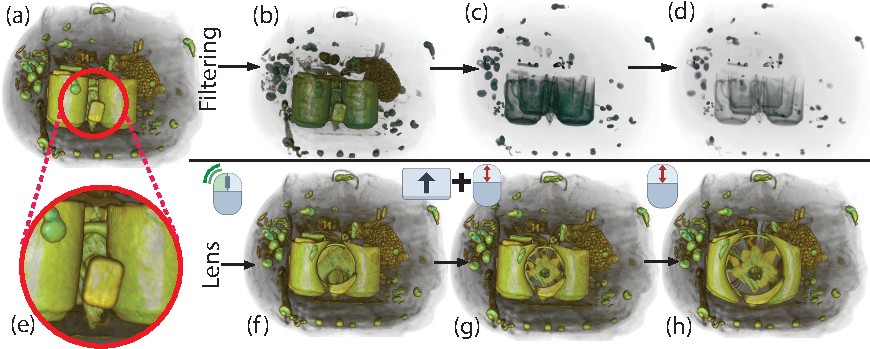
\includegraphics [width=\textwidth]{images/shuriken.eps}

\caption[Using our interactive lens on baggage.]{(a-c) A baggage scan is viewed from different angles. In view (c), a suspicious sharp object is spotted between a set of mugs. (d-f) Filtering densities using a classical 1D opacity transfer function removes progressively more of the occluders (mugs), but also the target. (g) The user applies the lens on the target object (double-click). An animation starts opening the lens, rays are gathered to pass through occluders. Halfway the animation, the object is magnified, but only the area close to the lens is visible. (h) The fish-eye field of view at the end of the animation scatters rays to fully show the target. (i) The lens is increased to magnify the target (mouse scroll).}
\label{f:baggage_lens}
\end{figure}


Baggage labeled as suspicious by human inspection or automated scan heuristics must be checked by human agents. Besides time-consuming physical unpacking, one can use 'virtual unpacking' tools that segment the 3D scan by a density-based confidence measure and next move the segmented objects away by animation to reduce occlusion\,\cite{Li:2012:LVV:2425296.2425325}. Such systems have been patented and used in production\,\cite{patent}. However, when the automatic segmentation is not optimal, the user must manually change its parameters, repeat the segmentation and animation, which goes back to being time-consuming.

Consider the baggage scan in \autoref{f:baggage_lens} ($283 \times 189 \times 344$ voxels, dataset obtained from an actual airport scan). Automatic baggage inspection systems will not detect anything suspect here. However, while visually exploring this baggage from different angles (\autoref{f:baggage_lens}a-c), we see an object hidden between a set of mugs. To reduce occlusion, a common solution in baggage inspection is to filter materials by density in order to show or hide subsets of the volume. However, for our dataset, the suspect target has almost the same density as the surrounding mugs, so removing the latter also removes the target (\autoref{f:baggage_lens}d-f). Using the obstruction-free fish-eye lens helps here: Clicking on the sharp detail visible in \autoref{f:baggage_lens}c first gathers rays so they pass through the low-density zone between the mugs (\autoref{f:baggage_lens}f). The animation that opens the lens 
(\autoref{f:baggage_lens}e-g) reveals an unobstructed view of the target. However, this shows only a small part of the target. Scattering rays next fully reveals the target (\autoref{f:baggage_lens}h). Adjusting the lens size shows a more detailed view of the target (\autoref{f:baggage_lens}i). Next, locally turning the viewpoint around the target (\autoref{f:rotation}) allows the agent to decide that the target is a shuriken (Japanese ninja star weapon). Since the object is very thick and blunt (see \autoref{f:rotation}), it is not an actual weapon, thus not a threat.

We evaluated our lens for this use-case by a user study. This evaluation is described bellow in \autoref{questanswers}.

\subsubsection{Early results}
\label{questanswers}

Eight airport security specialists were recruited (ages 23 to 43; experience in baggage scanning 8 months to 20 years; average familiarity with 3D tools, none considering him/herself an expert.


All attended a 20-minute global demo of the lens operation. Next, they were given each a personal training session for using the tool (5 minutes), in which they were instructed on the mouse and keyboard controls. After this, they were asked to work in pairs to examine the above-mentioned baggage CT dataset to form a decision on the nature of the ninja star possible threat (20 minutes of tool usage per person, after which the pair was changed). The idea behind this is that one person operates the tool while the other poses questions or suggest explorations, much like typical airport security operators work with a scanner. In the end, they all separately filled in a web questionnaire covering several questions and also provided open feedback (questionnaire available in the \autoref{AppendixA}). 


\autoref{questanswers} shows the answers. The first question-set (S1) regarded how easy-to-use, generally effective, and effective \emph{vs} other known tools our lens is for \emph{untargeted} inspection, \emph{i.e.}, when no suspect target is partially visible. Here and next, other tools denote classical 2D X-ray or 3D CT scans used in baggage scanning that the subjects know. As \autoref{fig:graph3}, \autoref{fig:graph4}, and \autoref{fig:graph5} show, 
the answers (on a 5-point Likert scale) were predominantly positive: The tool is easy to use, is useful, and is actually more useful than known tools for untargeted exploration. The second question-set (S2) regarded how good our tool is to examine \emph{specific} targets which are partially visible. Here again, the answers were predominantly positive (\autoref{fig:graph6}, \autoref{fig:graph7}, and \autoref{fig:graph8}). The main appreciated features of our tool are listed in \autoref{fig:graph9}.





\begin{figure}
\centering
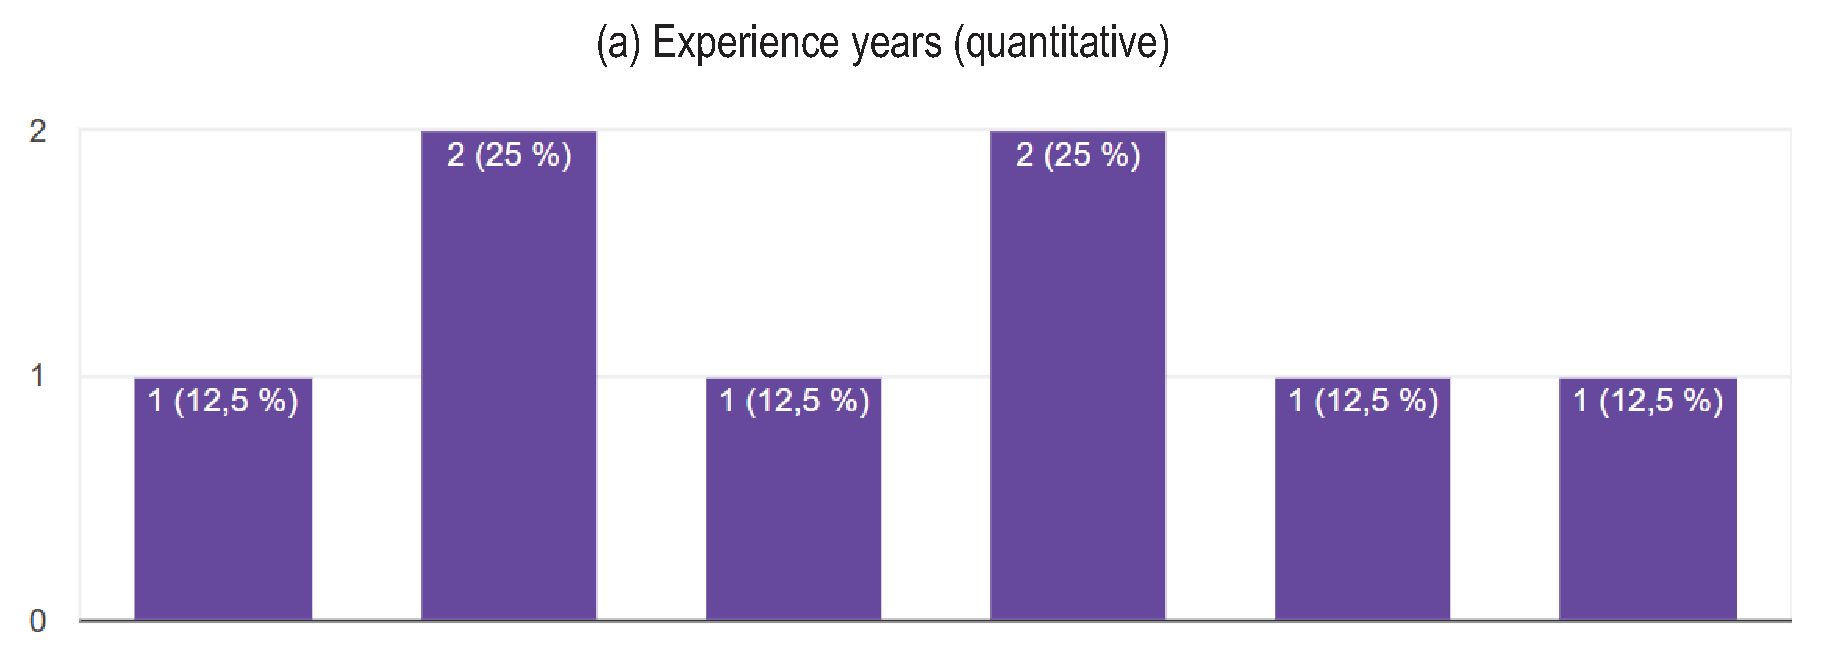
\includegraphics [width=\textwidth]{images/graph1.eps}
\caption{Evaluation of lens-based baggage inspection (\autoref{sec:baggage}): Experience years.}
\label{fig:graph1}

\end{figure}


\begin{figure}
\centering
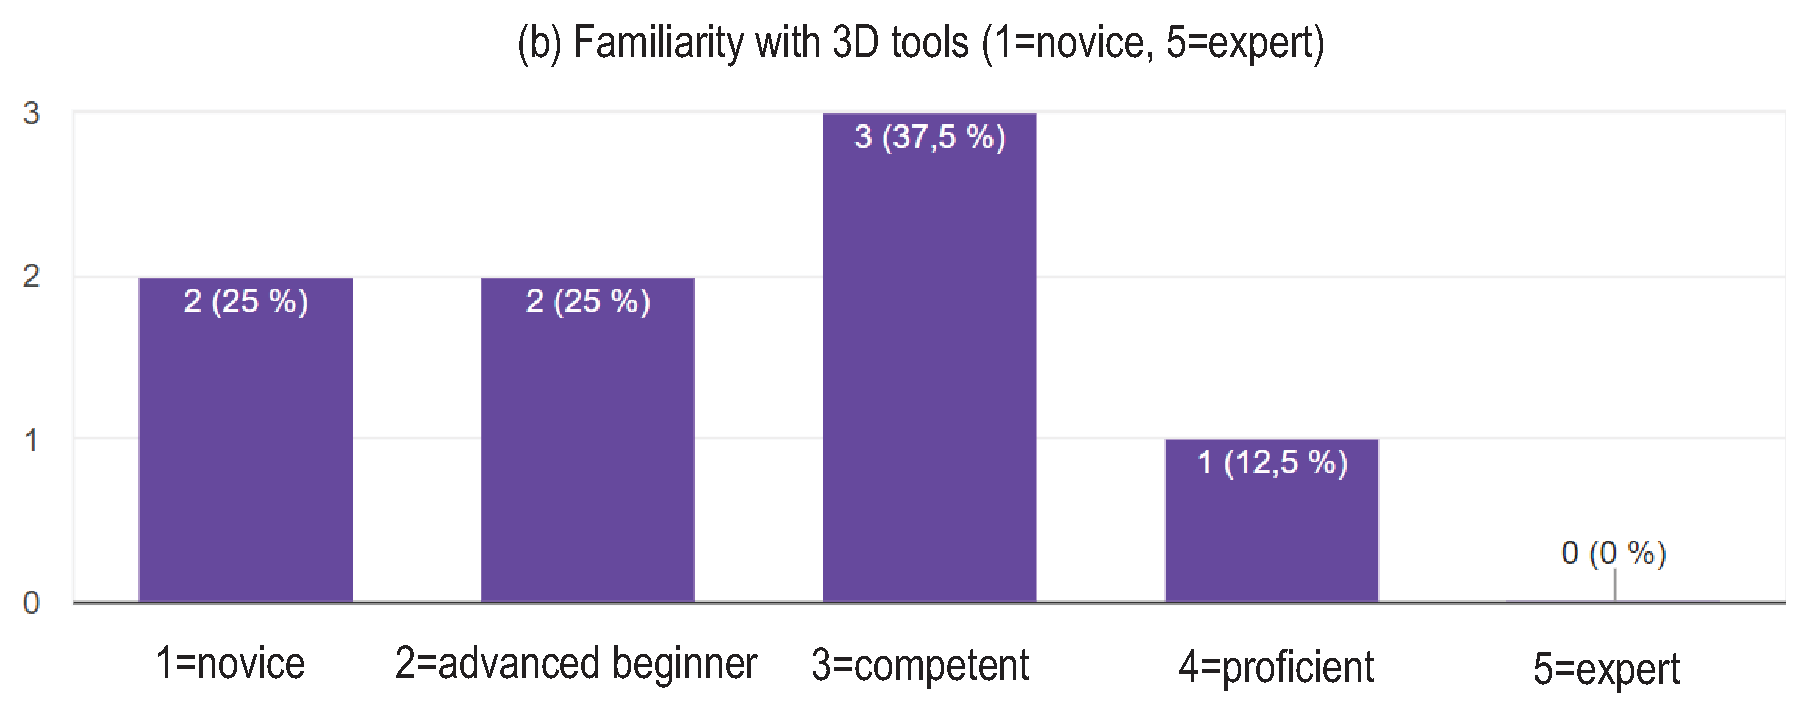
\includegraphics [width=\textwidth]{images/graph2.eps}
\caption{Evaluation of lens-based baggage inspection (\autoref{sec:baggage}): Familiarity with 3D tools.}
\label{fig:graph2}
\end{figure}


\begin{figure}
\centering
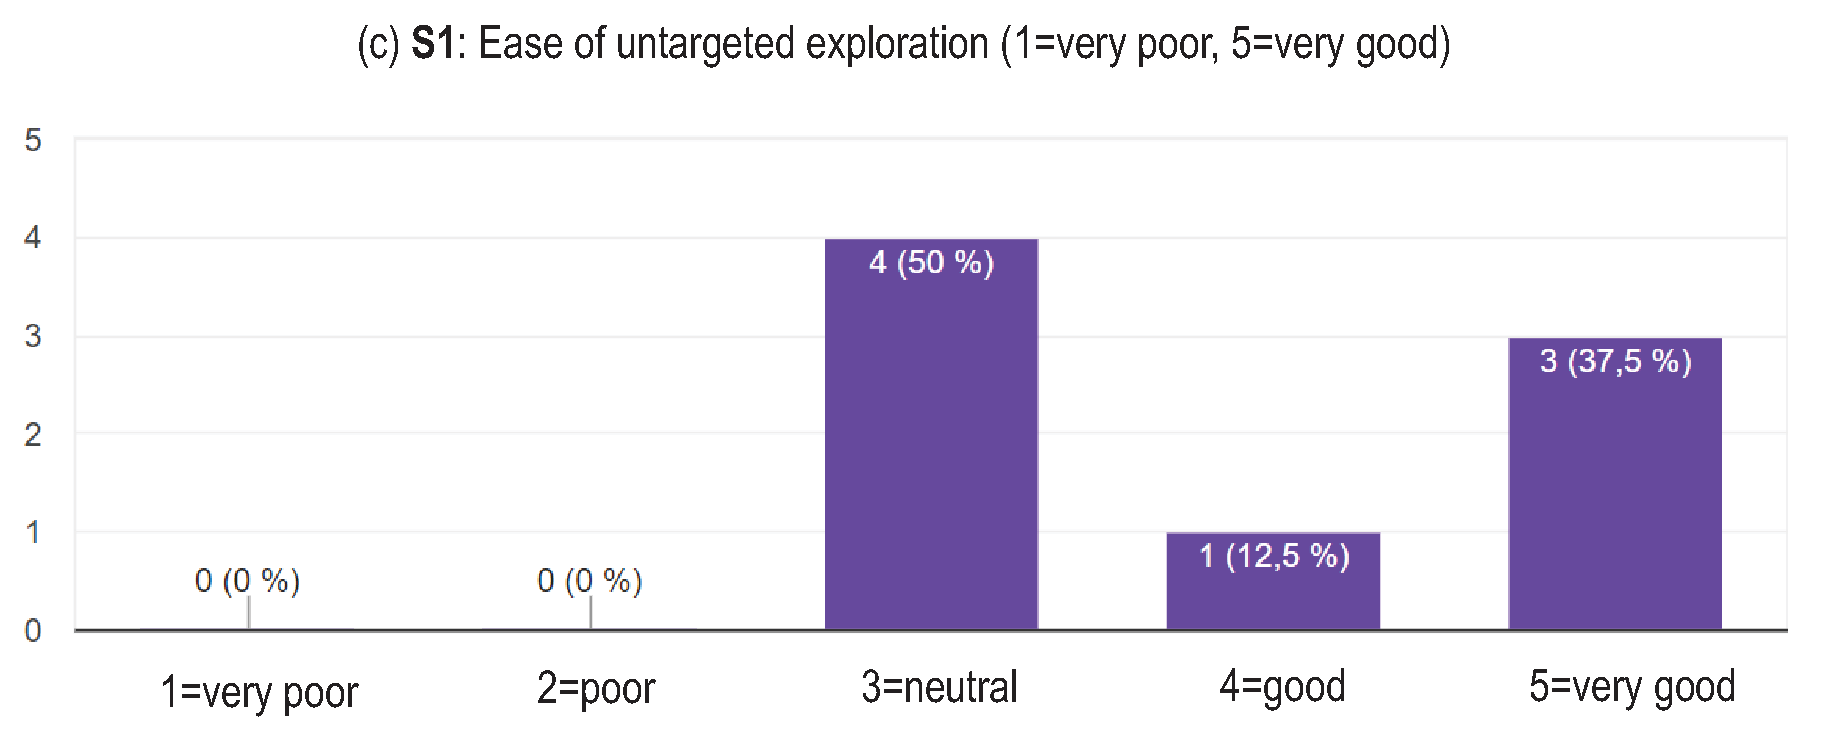
\includegraphics [width=\textwidth]{images/graph3.eps}
\caption{Evaluation of lens-based baggage inspection (\autoref{sec:baggage}): Scenario 1 - Ease of untargeted exploration.}
\label{fig:graph3}
\end{figure}


\begin{figure}
\centering
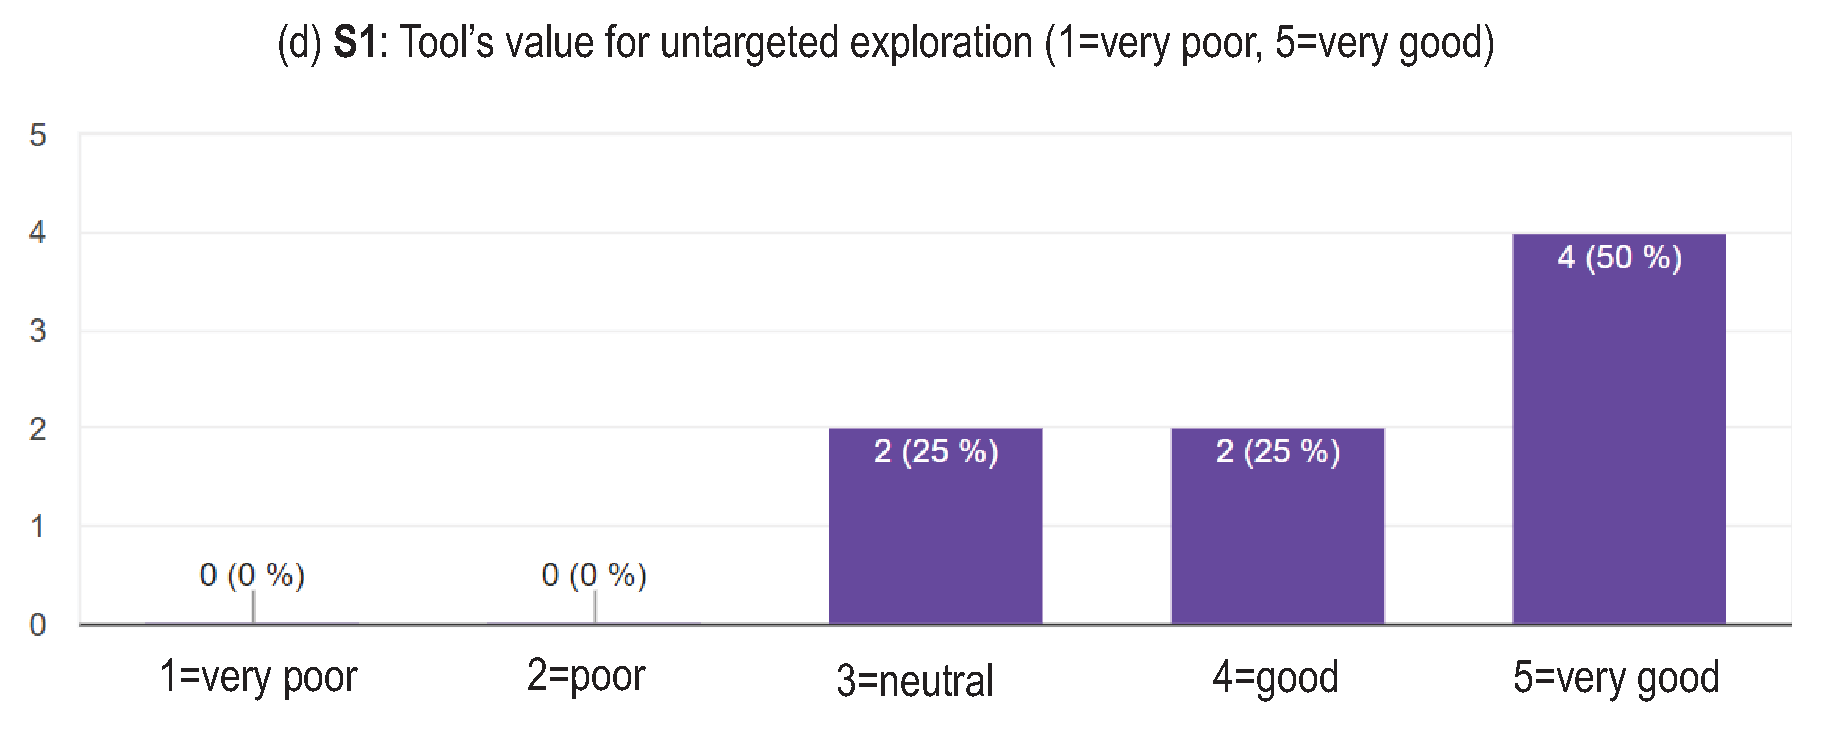
\includegraphics [width=\textwidth]{images/graph4.eps}
\caption{Evaluation of lens-based baggage inspection (\autoref{sec:baggage}): Scenario 1 - Tool's value for untargeted exploration.}
\label{fig:graph4}
\end{figure}

\begin{figure}
\centering
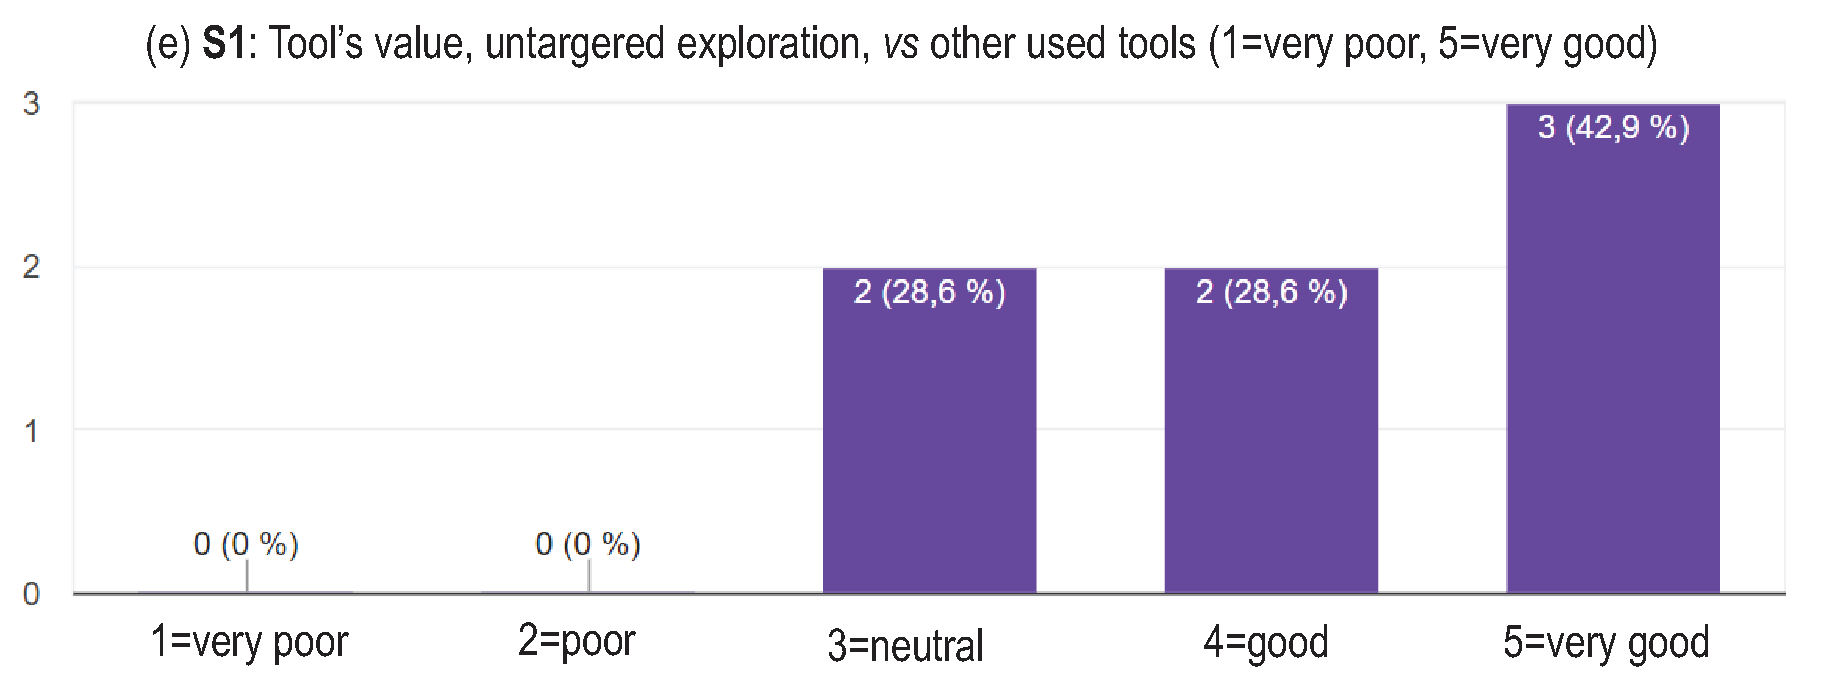
\includegraphics [width=\textwidth]{images/graph5.eps}
\caption{Evaluation of lens-based baggage inspection (\autoref{sec:baggage}): Scenario 1 - Tool's value, untargeted exploration, vs other used tools.}
\label{fig:graph5}
\end{figure}

\begin{figure}
\centering
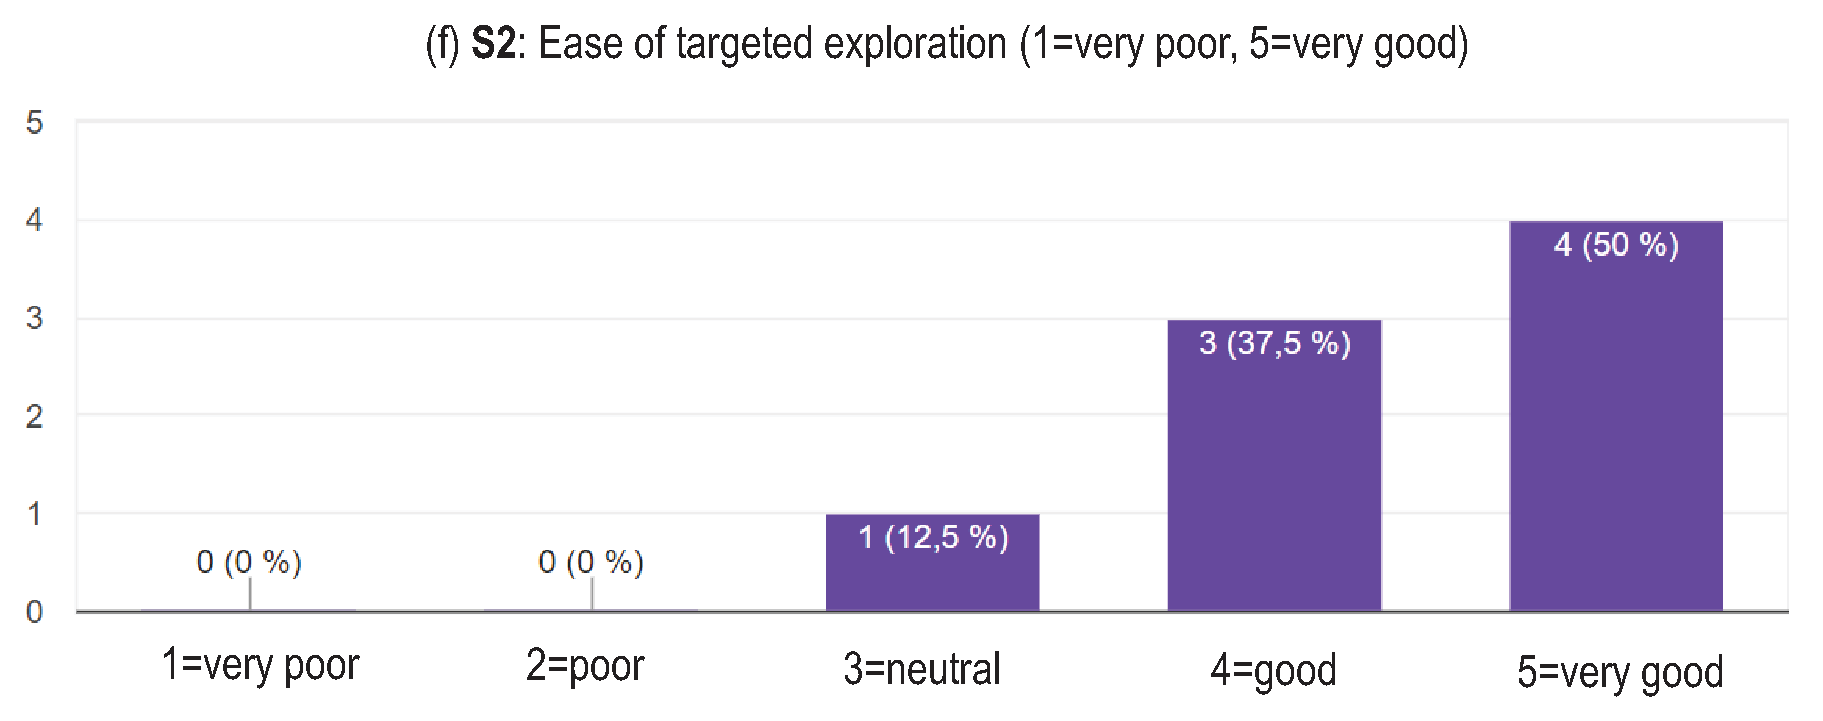
\includegraphics [width=\textwidth]{images/graph6.eps}
\caption{Evaluation of lens-based baggage inspection (\autoref{sec:baggage}) : Scenario 2 - Ease of untargeted exploration.}
\label{fig:graph6}
\end{figure}

\begin{figure}
\centering
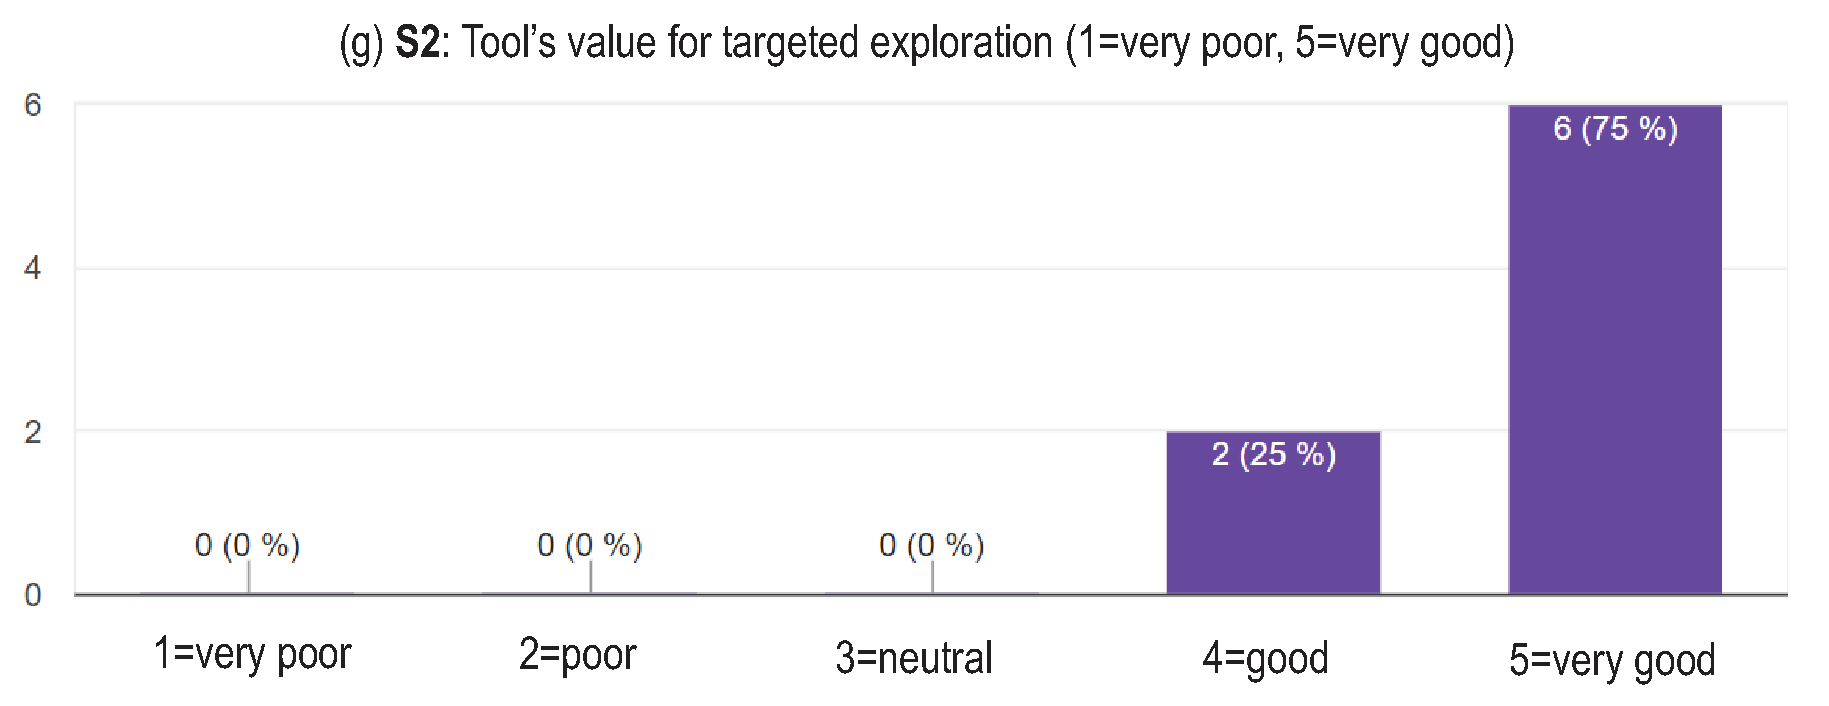
\includegraphics [width=\textwidth]{images/graph7.eps}
\caption{Evaluation of lens-based baggage inspection (\autoref{sec:baggage}): Scenario 2 - Tool's value for untargeted exploration.}
\label{fig:graph7}
\end{figure}

\begin{figure}
\centering
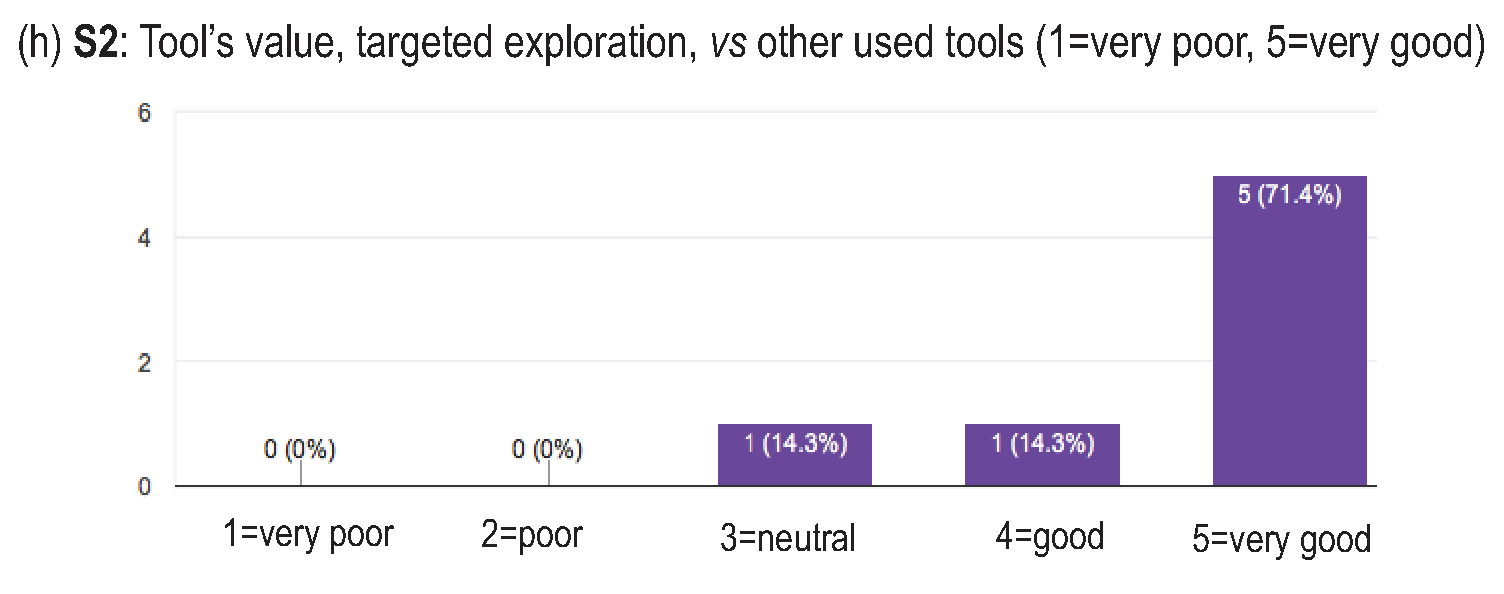
\includegraphics [width=\textwidth]{images/graph8.eps}
\caption{Evaluation of lens-based baggage inspection (\autoref{sec:baggage}): Scenario 2 - Tool's value, untargeted exploration, vs other used tools.}
\label{fig:graph8}
\end{figure}


\begin{figure}
\centering
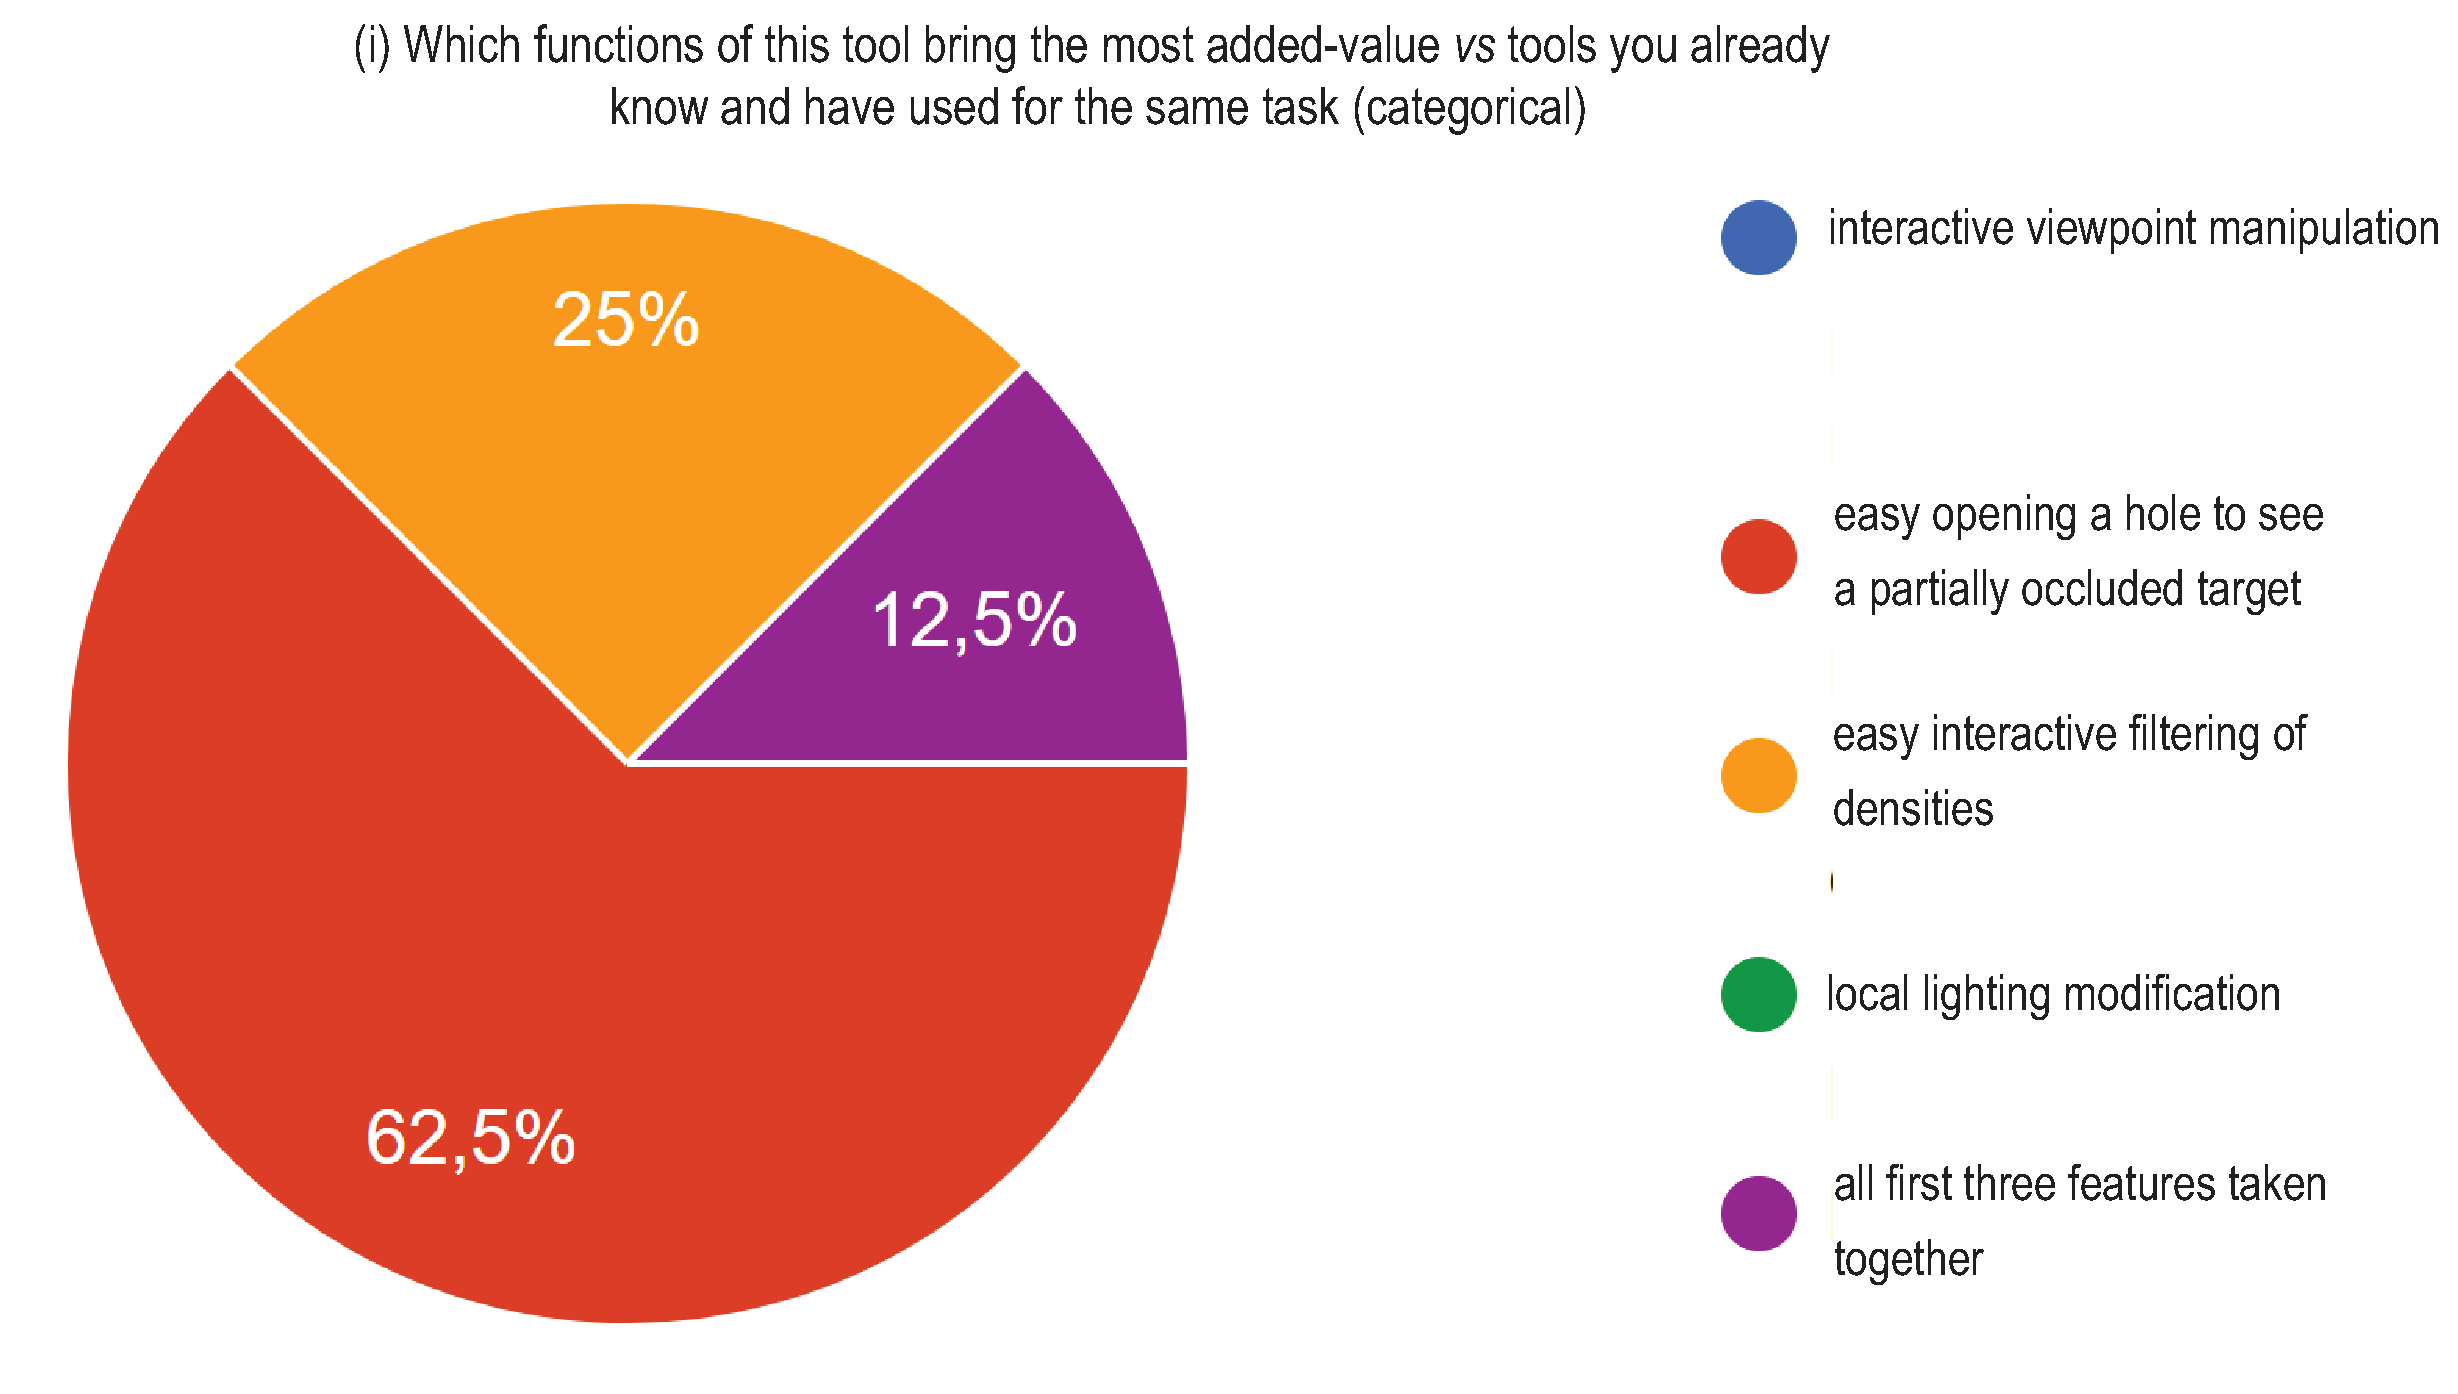
\includegraphics [width=\textwidth]{images/graph9.eps}
\caption{Evaluation of lens-based baggage inspection (\autoref{sec:baggage}): Which functions of this tool bring the most added-value vs tool you already know and have used for the same task (categorical).}
\label{fig:graph9}
\end{figure}


We next summarize the received open feedback. According to the subjects, our tool can provide them a better perception of the items inside the baggage as compared to the classical 2D single-viewpoint X-ray machinery they routinely use. Quotes from the open feedback: ''clear added-value compared to all systems I know''; ''this tool is a real gain for examining luggage with uniform and/or high densities''; ''definitely better than known tools for examining threats I am not familiar with / I have not seen before''. However, our tool should not be used for the typical carry-on baggage inspection which has a very small allowed inspection time (15 to 20 seconds). Our tool is much more interesting for inspecting checked-in baggage, where inspection time-windows are up to 3 minutes. The perceived added value for this use-case is also higher: Opening up checked-in baggage for manual inspection is much more complicated and time-consuming than for carry-on baggage. Moreover, the only system for inspecting checked-in baggage that the subjects knew of is a scanner that aims to \emph{automatically} detect threats via X-ray imagery; this system suffers from false positives, so a manual examination tool like ours could quickly eliminate such false positives, and thus the delays of opening up checked-in baggage. Finally, several subjects suggested that adding a function to display a classical 2D slice view (activated by a key press and aligned with the focal point) would be useful since this would show additional detail.


\subsection{Fluid flow: A deep-buried spherical vortex}
\label{sec:flow}
%
%
Flow visualization using streamlines has a long history\,\cite{brambilla2012illustrative,merzkirch2012flow}. For 3D datasets, a key challenge is to balance the streamline density. Low values allow seeing inner regions in the data but can subsample (miss) patterns. High values show more data but create too much occlusion. We next show how our lens can be used to alleviate problems in the latter case. The dataset\,\cite{griebel2004flow} captures the simulation of water flow in a basin computed on a grid of $128 \times 85 \times 42$ cells using 4595 streamlines with 183K sample points traced by pseudo-random seeding. We convert this set of 3D curves (polylines) to a scalar volume by using GPU-accelerated kernel density estimation (KDE)\,\cite{lhuillier2017ffteb}. Similar techniques have been used to compute density maps of 2D trail-sets\,\cite{hurter2012graph,cubu,hurter2015image}. 

We first explore the density volume ($500^3$ voxels) using standard DVR (\autoref{f:stream_lens}). Note that, given KDE's smoothing effect, streamlines appear as finite-thickness tubes rather than pixel-thin curves. After turning the viewpoint a bit, we notice a dense spherical item deep in the data (\autoref{f:stream_lens}a). To see its shape better, we increase opacity; however, this immediately increases occlusion so the item becomes invisible. Conversely, decreasing opacity to reduce occlusion makes the item almost transparent. Our lens solves the problem: In the initial view (\autoref{f:stream_lens}a), we point at the target and turn on the lens. This pushes away the occluding stream bundles, and shows that our item is a set of densely-packed, low-speed, tightly-turning streamlines that create a ball-like vortex (\autoref{f:stream_lens}b). 
To make sure our target is spherical, we view it in the lens from different directions, by interactively changing the ray directions in the lens (\autoref{f:stream_lens}c). Finally, we can close the lens but keep the target magnified (\autoref{f:stream_lens}d).
Finding the details of this vortex cannot be done using standard DVR. Interestingly, this vortex has also not been discovered by any of the visualization techniques that used this dataset (according to our knowledge) \,\cite{telea_vis_99,griebel2004flow,ddh,lhuillier2017ffteb}. 

\begin{figure}
\centering
\includegraphics [width=\textwidth]{images/stream_lens.eps}

\caption[Flow volume exploration with two different opacity transfer functions (top and bottom rows).]{Flow volume exploration with two different opacity transfer functions (top and bottom rows). In viewpoint (a), we notice a small high-density spherical item. (b) We apply the lens at that location (double click). (c) The directions of rays in the lens are changed to see the whole target in the lens (right click + mouse drag change direction). (d) The lens is gradually closed while keeping the focus area magnified (shift + scroll).}

\label{f:stream_lens}
\end{figure}

\subsection{Chest scan: A hard to see tumor}
\label{sec:chest}
%
In our third use-case, we consider a contrast chest CT scan ($512 \times 512 \times 110$ voxels) of an elderly patient with a sizeable lung tumor. The tumor was detected in a CT scan performed after the patient reported acute chest pain. Typical examination of these scans by the pulmonologist and radiologist in charge involves slice-based views. \autoref{f:slicer}a-c and \autoref{f:slicer}d-f show two such slice sets (axial, coronal, and sagittal views), produced using typical lung, respectively mediastinal, contrast presets.

 Although the tumor is visible in all these views, its exact shape, morphology, and connection to the lung walls are hard to assess. Finding such details on the tumor is essential, explained the doctors in charge, to determine the TNM score\,\cite{brierley} and also planning treatment. Using standard DVR makes the tumor and its 3D position partially visible (\autoref{f:slicer}f). Yet, occlusion from the rib cage and other tissues is still present. Using both TF presets and manually changing the TFs in the 3D Slicer tool\,\cite{slicer} used to create the DVR could not help de-occluding the tumor without making it partly transparent.
 
  The slice images in \autoref{f:slicer}a-f confirm this by showing that the gray values for the tumor and surrounding skin-and-muscle tissue are very similar. This is due to the fact that the tumor had grown rapidly and started necrotizing, which filled it with fluids, making its density very similar to that of the obstructing (skin and muscle) tissue, explained the pulmonologist. Hence, one cannot remove such occluding tissue in a classical DVR setting by opacity TF manipulation without also removing the tumor. This makes examining this specific tumor harder than for regular cases.

\begin{figure}
\centering
\includegraphics [width=\textwidth]{images/slicer.eps}
\caption[Lung tumor visualization using slices and standard DVR.]{Lung tumor visualization using slices (a-c) and standard DVR (d). Annotations are manually added by the examiner to delineate the tumor location. Images constructed using the 3D Slicer tool\,\cite{slicer}.}
\label{f:slicer}
\end{figure}

We next used our lens to examine the tumor. \autoref{f:params} shows several sample snapshots. We see that the tumor is significantly more visible when using the lens than when using standard DVR (\autoref{f:slicer}d), both in terms of removing the occluding tissue and in terms of the tumor's opacity -- compare the inset in \autoref{f:slicer}d with the images in \autoref{f:params}. Secondly, relighting the tumor from various directions allows one to see small-scale morphological details such as the tumor's surface shape and its connection via protuberances and veins with the lung walls.

We asked the two medical specialists (pulmonologist and radiologist) in charge to state the potential advantages and/or limitations of our lens as compared to standard slicing and DVR techniques, after a 20-minute usage of the tool. 
Both specialists have over 10 years of medical experience in treating lung cancer, and routinely use several slicing and DVR tools. They work in a private hospital in Belgium and are not actively associated with medical imaging research. Our identities were hidden from them during the lens evaluation. The provided input can be summarized as follows: The occlusion-free lens is definitely easier and faster to use than classical DVR and/or slicing techniques. It is especially more effective than these to get a quick, first impression of a deep buried anatomical detail. Changing the lens' parameters by direct interaction is as simple as changing window/level functions in a typical slice-based tool, and is definitely simpler than tuning typical DVR parameters to obtain similar results. This 'entices' the user to explore, which is a good aspect. The fact that the lens minimizes viewpoint change (volume rotation), \emph{i.e.}, after a suitable viewpoint was found from which a (small) part of the target is visible, one doesn't need to change this viewpoint, is a strong feature, as 3D viewpoint changes are disruptive and cost time. This is important in a cost-aware environment where specialists have very limited time (about 20 minutes) to assess a CT scan. However, the lens should not \emph{replace} classical slice-based exploration, which shows small-scale details better. In the context of the current dataset (\autoref{f:slicer}), the lens was useful to both confirm the TNM score (T3 grade tumor, 6.5 cm in size) found via the 2D slices, but much more so for understanding how and where the tumor is connected to surrounding tissue, which is very hard to do using only 2D slices.

\begin{figure}
\centering
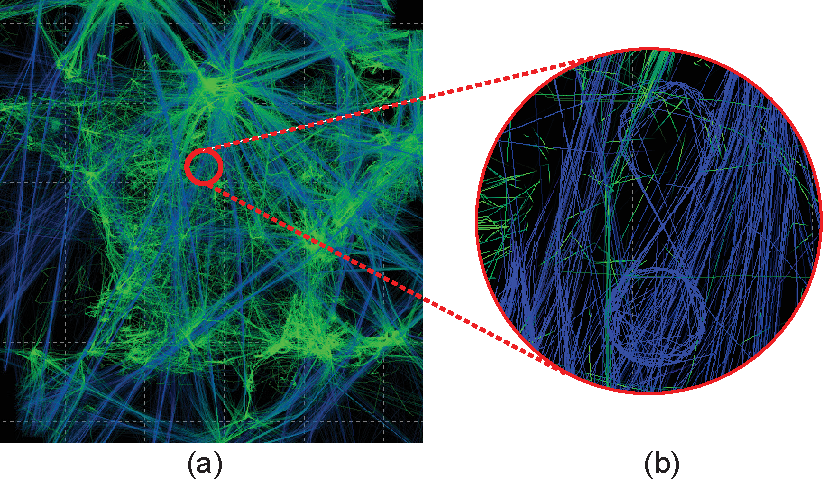
\includegraphics [width=\textwidth]{images/aircraft.pdf}

\caption[Visualizing one day of aircraft trajectories over France.]{Visualizing one day of aircraft trajectories over France\,\cite{hurter2009fromdady}. (a) Overview of all trails. (b) Zoom, filtering, and color mapping techniques are used to highlight an outlier trajectory of an aircraft performing an eight-shaped loop. Revealing this outlier costs significant user effort.}
\label{f:fromdady}

\end{figure}


\subsection{Aircraft trajectories: Outliers in the French sky}
\label{sec:atc}
%
%
We next consider a task from air traffic planning -- detecting and studying outliers in large-scale datasets containing tens of thousands of 3D (latitude, longitude, height) trails of aircraft over a given spatio-temporal region\,\cite{hurter2014interactive}. Such datasets are typically viewed using 2D (latitude, longitude) plots where opacity encodes the spatial density of flights -- see \autoref{f:fromdady}a, which shows one day of recorded aircraft trajectories over the French airspace. \autoref{f:fromdady}(b) shows a detail zoom-in, where we can see an abnormal -- that is, far from straight or slightly curved -- aircraft trail: A tanker aircraft performed an eight-shaped loop as it was waiting to refuel other aircraft. Revealing such patterns using 2D techniques, \emph{e.g.} \cite{hurter2009fromdady}, is very hard. In particular, it is hard to de-occlude these patterns from the overall context of criss-crossing aircraft trails, even when one knows their 2D spatial location.

Our lens can help with this task, as follows. We first convert the set of 3D trails to a $500^3$ density volume, using KDE as for the streamline use-case (\autoref{sec:flow}). Examining this volume via standard DVR shows an outlier trail at some point in space, see curved patterns in \autoref{f:aircraft_lens}a. Activating the lens on this area and interactively tuning the target depth $t_{min}$ (since we don't know the trail's height) beings the outlier trajectory in focus and pushes away occluding trails (\autoref{f:aircraft_lens}a). Like in the other examples presented so far, we can quickly change the magnification factor and view direction to better study this trail in context (\autoref{f:aircraft_lens}b-d). From these images, we easily see that the outlier trail has an eight shape. Revealing this outlier trail using standard 2D visualization techniques\,\cite{hurter2009fromdady} costs several minutes. Doing the same using our lens costs under one minute. Also, comparing \autoref{f:fromdady}b and \autoref{f:aircraft_lens}b-d, we argue that the eight-shape of the outlier trail is much more prominent, and thus recognizable, in the latter images (made using our lens) than in the former ones. Last but not least, the 3D DVR approach that our lens enhances explicitly encodes flight height information, so our lens can use it by interactively tuning the depth value $t_{min}$ where the lens is focused. This cannot be done with 2D techniques which ignore the depth dimension.

We validated our findings with an air traffic data scientist with more than 10-year experience in air traffic control and planning. She confirmed that this specific eight-shape trail in \autoref{f:fromdady}(b) is an actual aircraft which performed waiting loops and acted as a fuel supplier for military aircraft. Other comments included the following: Compared to standard 2D visualization techniques, our tool makes detecting outliers easy since there is no need for complex manipulation to reveal such outlier trails. Also, the user does not have to deal with color and alpha mapping parameter-tuning to make specific outliers emerge. Separately, trail visualization easily creates many occlusions leading to either fully opaque areas or too much local overlap, which both hinder seeing and examining specific trails. Our lens does help such cases by distorting the space to locally remove such occlusions. All in all, in the studied dataset (\autoref{f:fromdady}), the lens was specifically useful since, for high transparency, one would not detect the outlier trail, while for low transparency, one would get a hint of the outlier's existence, but not see it in detail due to too much occlusion; the lens allows using low transparency, but removes the clutter caused by it to reveal the outlier.


\begin{figure}
\centering
\includegraphics [width= \textwidth]{images/aircraft_lens.pdf}
\caption[Inspecting an abnormal aircraft trail.]{Inspecting an abnormal aircraft trail. (a) The abnormal trail is spotted in an all-trails view as it is highly curved while all other trails are relatively straight. Activating the lens at the outlier location (b) and changing the magnification factor (c) reveals the trail's eight-shape. (d) Rotating the viewpoint provides spatial insight on the embedding of the outlier in the surrounding trails.}
\label{f:aircraft_lens}
\end{figure}
%

\subsection{Brain fibers: Uncluttering the bridge}
\label{sec:dti}
%
Our last use-case considers the exploration of fiber tracts visualized as streamlines of the major eigenvector of a diffusion tensor imaging (DTI) field. Such datasets have a spatially complex structure which makes them hard to explore\,\cite{assaf08}. In particular, fiber tracts are spread volumetrically over the entire extent of the brain, and create tangled patterns inside which it is hard to see much. DVR techniques are often used to render such tracts, one of the advantages being that close fibers get visually 'merged' to reveal spatially coherent structures, an effect which is not possible when fibers are rendered as polylines. However, DVR methods also create more occlusion, thus difficulties in seeing structures deep within the volume.

We consider an $128 \times 128 \times 51$ DTI volume (same dataset as in\,\cite{everts15}). We traced 150352 fibers seeded in, and going over, regions of high fractional anisotropy in this volume. We filtered out fibers shorter than 2mm, yielding a total of 120593 fibers to display (6.4M sample points). Next, we converted this fiber-set to a $512^3$ density volume, using KDE with a 3D isotropic kernel of radius 15 voxels, like for the streamline use-case (\autoref{sec:flow}). \autoref{fig:dti}a shows the result, rendered with DVR, with opacity function mapping the fiber density. While terminal fibers are well visible, we cannot see anything inside the volume. Activating the lens in the middle of the volume opens a hole through which a small part of the \emph{corpus callosum}, the fiber bundle wrapping the bridge that connects the two hemispheres, becomes visible. By slightly decreasing opacity (\autoref{fig:dti}c), the \emph{corpus callosum} gets clearly visible, appearing as a compact structure, due to the KDE blending of neighbor fibers. Obtaining such a view of the \emph{corpus callosum} only using DVR would be very hard, since transfer functions would either render separated (non-merged) fibers, or else make the fibers surrounding the structure of interest too thick and occluding. 

This scenario has the main difference compared to all previous ones. In all earlier cases, the standard DVR of the data (that is, without the lens) showed us a partial small cue of the structure of interest within the volume, and we used the screen-space location of this structure as the focus point where to activate the lens. In this last scenario, there is no point in the original DVR image (\autoref{fig:dti}a) from which the \emph{corpus callosum} is even partially visible, due to the high opacity given by the used transfer function. Hence, the user can activate the lens at \emph{any} desired point to peek inside, and towards the center of, the volume. Given the nature of the data, the structure of interest is quite easily visible from most such viewpoints (see lens inset in \autoref{fig:dti}b). Once its presence is revealed, the user can next adjust the viewpoint and/or the opacity transfer function to get an optimal view on the target, such as the one shown in \autoref{fig:dti}c. Summarizing, we can use our lens also in cases when no partial view of a target is available. 

\begin{figure}
\centering
\includegraphics [width=\textwidth]{images/dti.eps}
\caption{Revealing the \emph{corpus callosum} in a DVR of a set of DTI tracts.}
\label{fig:dti}
\end{figure}

%
\section{Discussion}
\label{sec:discussion}
%
%
Several points of our lens proposal are worth discussing, as follows.


\par \textbf{Lens activation:} Our lens can support two types of explorations. First, when the user perceives a \emph{part} of a target of interest in a classical DVR image, the lens can be used to reveal the target in full detail. This \emph{directed} exploration supports the task `show me more information about \emph{this} item'. The use-cases in \autoref{sec:baggage}-\autoref{sec:atc} are of this type. Secondly, the user can open up a DVR volume at a 2D location from which no partial detail is visible. This is useful when we know that there \emph{is} an interesting target buried in the volume even without seeing it (\emph{corpus callosum} use-case in \autoref{sec:dti}), thus supports the task `show me the data I \emph{know} it is somewhere in there', or for free exploration to find unknown patterns in a volume, \emph{i.e.} for the task `show me what this volume \emph{may} hide in it'. In the first exploration type (target not fully occluded), our lens is simple and rapid to use -- point, click, and optionally rotate light or viewpoint. In the second exploration type (target fully occluded or not even sure whether an interesting target exists in the data), the lens is equally simple to use, but several tries to select a suitable focus point and lens depth are needed.

\par \textbf{Lens shape:} Occluders are pushed away, and deformed, isotropically (\autoref{sec:scattering}, \autoref{continuity}). This simple lens model requires a single parameter, the lens radius $R$, which makes its usage easy. The deformations evolve smoothly from the lens center (maximal) to outside the lens (no deformation), see \autoref{continuity}, which effectively blends the local (in lens) focus with the global (out of lens) context (R3). However, this strongly compresses the deformed occluders close to the lens border, making them hardly visible when the lens is fully active. A possible refinement would be to reduce the deformation of the pushed-away occluders while still pushing them away, thereby improving the F+C effect (R3). However, this would occlude areas outside the lens, basically moving occlusion from \emph{inside} the lens to \emph{outside} and close to it. Finding an optimal balance between minimal deformation (so one can recognize the pushed-away occluders) and minimal clutter (so these occluders do not destroy the lens context) is a topic for future work. Separately, deformed rays may intersect with straight rays, thereby sampling the same voxel(s) to different image pixels. We did not observe in our usage any artifacts that can be ascribed to this issue, nor did the other users of our tool. This can be explained by the fact that such ray intersections are relatively few and we use a compositing transfer function, akin to a low-pass filter.


\par \textbf{Parameter setting:} Our lens depends on several parameters: the 2D lens center $\mathbf{f}$, lens radius $R$, lens axis direction $\mathbf{a}$, local light direction $\mathbf{l}^{lens}$, scattering start-distance $t_{min}$, and gathering and scattering parameters $\alpha$ and $\beta$. All these parameters are controlled via a mouse-driven virtual trackball, key modifiers, and the arrow keys (\autoref{sec:principle}). As the lens works at 15 frames per second, the user can quickly tune the parameters and see their effect (R1). Moreover, all parameters start with good preset values (\autoref{sec:principle}). A possible refinement would be to pre-segment the target, based on user-given values for $\mathbf{f}$, $R$, and $t_{min}$, thereby determining $\beta$ automatically. However, we believe that manual control of the scattering $\beta$ is important to allow users to choose their most suitable field-of-view angle. In fact, this flexibility allows a better exploration of the local context (R2).


\par \textbf{Implementation:} We implement our lens by modifying the ray trajectories constructed in the inner loop (per-pixel raycasting) of a public DVR raycaster\,\cite{cudasdk}. Apart from this, we change the per-voxel lighting and transfer function based on the voxel location in the lens and the parameters given by user interaction (\autoref{sec:inter_expl}). Such changes are limited and easily applicable to any (parallel) raycaster.


\par \textbf{Limitations:} As explained, de-occluding a target requires either a small fragment thereof to be visible (if so, de-occlusion is very simple and fast), or requires the user to choose the lens focus and target depth based on other insights (which, as explained, requires more trial-and-error). At a higher level, many lens mechanisms exist in the literature, as discussed in \autoref{sec:requirements}. While we have argued that, to our knowledge, none of them simultaneously supports requirements R1,$\ldots$,R4, comparing such mechanisms with our lens for specific use-cases and datasets is an important test for the \emph{end-to-end} effectiveness of our proposal. We have not covered this point as obtaining (or replicating)  implementations of such lenses is very challenging. This remains an important open point for future work -- both for our proposal but also for all other volumetric lens proposals in the literature. In particular, none of the techniques in \autoref{tab:methods} were compared side-by-side against other techniques. We have performed three user evaluations involving specialists in airport baggage security (\autoref{sec:baggage}), pulmonology (\autoref{sec:chest}), and air traffic control (\autoref{sec:atc}). In all cases, users were not involved in this work, nor with other work of the authors. However, the set-up of these evaluations stays at the level of formative user experiments. To confirm and refine the obtained (positive) findings, more formal user studies are needed, which we plan to cover next.

\section{Conclusions}
\label{sec:conclusions}
%
In this chapter, we presented a new fish-eye-like context-and-focus lens that addresses the occlusion problems inherent in scalar volume rendering. The principle of our lens consists in first gathering (squeezing) rays so that they easily pass through occluding densities (given a user-specified opacity transfer function) and next scattering (fanning out) rays to best sample the target of interest. Our lens can be directly applied to any DVR raycaster and scalar volume dataset. Its main constraint is that the user should be able to find a viewpoint from which the target of interest, deep buried in the data, is at least slightly visible. We also present several modifications of the local rendering parameters within the lens (view direction, lighting parameters, opacity transfer function) that aim to both better separate the focus (lens) from the context (volume) and also allow more detailed examining of the target. Our lens is easy to use -- all its parameters are controlled via direct mouse-and-keyboard interaction -- and can be efficiently implemented atop of a standard GPU ray caster. Our lens is especially useful for highlighting structures of interest which are both deeply embedded in volumetric data and cannot be revealed by standard transfer function manipulations due to similar densities in the occluders and target. We demonstrate these points using five use-cases involving datasets from baggage detection, fluid visualization, air traffic control, and chest radiology, and DTI fiber tracts.

Several improvements to our proposal are possible, as follows. First and foremost, heuristics can be sought to link all our free parameters (lens size, focus depth, interpolation between focus and context) directly to the volume data, so the user interaction is minimized and therefore exploration efficiency is increased. Secondly, our lens could be extended to different types of volumetric datasets, such as multivariate (vector, tensor) fields. Last but not least, a formal wider-scale evaluation of how the lens addresses more specific tasks, and how it compares to existing tools for these tasks, such as other lens types, is a goal we aim to pursue next.